\documentclass{beamer}
\usetheme{CambridgeUS}
\usefonttheme{serif}

\usepackage{amsmath}
\usepackage{amsfonts}
\usepackage{geometry}
\usepackage{float}
\usepackage{algorithmicx}
\usepackage{algorithm}
\usepackage{tikz}
\usetikzlibrary{arrows}
\usepackage{listings}
\usepackage{xcolor}

\newcommand{\tensor}[1]{\mathbf{#1}}
\newcommand{\dV}{\,\mathrm{d}V}


\title[YAFEL]{Yet Another Finite Element Library}
\author{Tyler Olsen}
\date{June 30, 2016}

\AtBeginSection[]{
  \begin{frame}{Outline}
    \tableofcontents[currentsection]
  \end{frame}
}


%===========================================================
%===========================================================
\begin{document}


\begin{frame}
  \titlepage
\end{frame}

\section{FEM Overview}
%===========================================================
\subsection{Problem}
%===========================================================
\begin{frame}{Example Problem: Heat Equation}
  \begin{itemize}
  \item
    Demonstrate FEM using steady-state heat equation (omitting technical details)
    \begin{align*}
      \nabla^2 u &= 0 &\forall \;\;\tensor{x}&\in \Omega \\
      u &= \hat{u}(\tensor{x}) &\forall \;\;\tensor{x} &\in \partial \Omega_D \\
      \nabla u \cdot \tensor{n} &= g(\tensor{x}) &\forall \;\; \tensor{x} &\in \partial \Omega_N
    \end{align*}
  \item
    As written, this PDE applies point-wise throughout the domain $\implies$ ``Strong Form''
  \end{itemize}
\end{frame}


%===========================================================
\begin{frame}{Weak Form}

  \begin{itemize}
  \item
    For FEM, we transform the PDE to the ``weak form''
  \item
    Multiply by a ``test function'' $v$ that satisfies boundary conditions and 
    certain integrability requirements, then integrate by parts
    \begin{align*}
      \int_{\partial \Omega_N} v (\nabla u \cdot \tensor{n})\,\mathrm{d}A - 
      &\int_{\Omega} \nabla v \cdot \nabla u \dV = 0  \\
      &\forall\;\; v \in 
      \{\text{a set satisfying above requirements}\}
    \end{align*}
  \end{itemize}

\end{frame}


%===========================================================
\subsection{Spatial Discretization}
%===========================================================
\begin{frame}{Discretize Domain}

  \begin{columns}
    \begin{column}{.5\textwidth}
      \begin{itemize}
      \item
        Express integrals over whole domain as sum of integrals over elements
        \begin{align*}
          \int_\Omega \nabla v \cdot &\nabla u \dV = \\
          &\sum_e \int_{\Omega_e} \nabla v \cdot \nabla u \dV
        \end{align*}
      \end{itemize}
    \end{column}
    \begin{column}{.5\textwidth}
      \begin{figure}
        \centering
        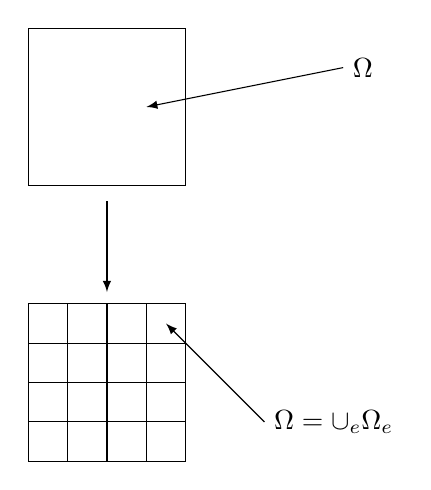
\begin{tikzpicture}[scale=2.0]
          %original box
          \draw (0,0) -- (1,0) -- (1,1) -- (0,1) -- (0,0);
          
          \draw[latex-] (.75, .5) -- (2,.75) node[right]{$\Omega$};
          
          % down arrow
          \draw[-latex] (0.5, -0.1) -- (0.5, -0.675);

          \draw (0,-1.75) -- (1,-1.75) -- (1,-0.75) -- (0,-0.75) -- (0,-1.75);
          \draw (0,-1.5) -- (1,-1.5);
          \draw (0,-1.25) -- (1,-1.25);
          \draw (0,-1) -- (1,-1);
          \draw (0.25,-0.75) -- (0.25,-1.75);
          \draw (0.5,-0.75) -- (0.5,-1.75);
          \draw (0.75,-0.75) -- (0.75,-1.75);
          \draw[latex-] (.875, -0.875) -- (1.5,-1.5) node[right]{$\Omega = \cup_e \Omega_e$};
        \end{tikzpicture}
      \end{figure}
    \end{column}
  \end{columns}

\end{frame}


%==============================================================
\begin{frame}{Change of integration bounds}

  \begin{columns}
    \begin{column}{0.5\textwidth}
      \begin{itemize}
      \item
        Generally, elements are not regular rectangles, so
        we change bounds of integration to an easier element
        shape to integrate over
      \item
        This easier shape is called the ``parent'' or ``canonical'' element
      \item
        For quadrilaterals, the canonical element is $\Omega_0 = [-1, 1] \times [-1, 1]$
      \end{itemize}
    \end{column}
    \begin{column}{0.5\textwidth}
      \begin{figure}
        \centering
        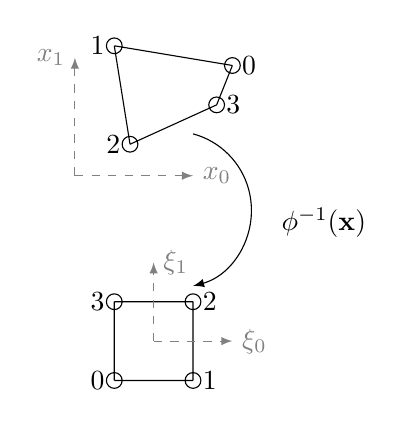
\begin{tikzpicture}{scale=2.0}
          
          \draw (0,0) circle[radius=.1] node[left]{0}-- 
          (1,0) circle[radius=.1] node[right]{1} -- 
          (1,1) circle[radius=.1] node[right]{2} -- 
          (0,1) circle[radius=.1] node[left]{3} -- (0,0);
          \draw[color=gray, dashed, -latex] (0.5,0.5) -- (1.5,0.5) node[right]{$\xi_0$};
          \draw[color=gray, dashed, -latex] (0.5,0.5) -- (0.5,1.5) node[right]{$\xi_1$};
          
          \draw (.2,3) circle[radius=.1] node[left]{2}
          -- (1.3,3.5) circle[radius=.1] node[right]{3}
          -- (1.5,4) circle[radius=.1] node[right]{0}
          -- (0,4.25) circle[radius=.1] node[left]{1}
          -- (.2,3);
          \draw[color=gray,dashed, -latex] (-0.5, 2.6) -- (1, 2.6) node[right]{$x_0$};
          \draw[color=gray,dashed, -latex] (-0.5, 2.6) -- (-0.5, 4.1) node[left]{$x_1$};
          
          \draw[latex-] (1,1.2) arc (-75:75:1);
          \draw (2,2) node[right]{$\phi^{-1}(\tensor{x})$};
          
        \end{tikzpicture}
      \end{figure}
    \end{column}
  \end{columns}

\end{frame}


%==============================================================
\begin{frame}{Change of integration bounds}

  \begin{columns}
    \begin{column}{0.5\textwidth}
      \begin{itemize}
      \item
        The transformation results in:
        \begin{align*}
          \int_{\Omega_e}\nabla v \cdot &\nabla u \dV = \\
          &\int_{\Omega_0}\nabla v \cdot \nabla u \;\mathrm{det}(\tensor{J})\dV_0 \\
          %
          %
          \\
          \text{Where } &\tensor{J} = \frac{\partial \tensor{\phi}}{\partial \tensor{\xi}} > 0
        \end{align*}
      \end{itemize}
    \end{column}
    \begin{column}{0.5\textwidth}
      \begin{figure}
        \centering
        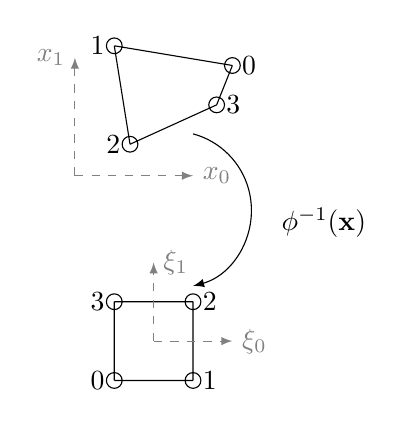
\begin{tikzpicture}{scale=2.0}
          
          \draw (0,0) circle[radius=.1] node[left]{0}-- 
          (1,0) circle[radius=.1] node[right]{1} -- 
          (1,1) circle[radius=.1] node[right]{2} -- 
          (0,1) circle[radius=.1] node[left]{3} -- (0,0);
          \draw[color=gray, dashed, -latex] (0.5,0.5) -- (1.5,0.5) node[right]{$\xi_0$};
          \draw[color=gray, dashed, -latex] (0.5,0.5) -- (0.5,1.5) node[right]{$\xi_1$};
          
          \draw (.2,3) circle[radius=.1] node[left]{2}
          -- (1.3,3.5) circle[radius=.1] node[right]{3}
          -- (1.5,4) circle[radius=.1] node[right]{0}
          -- (0,4.25) circle[radius=.1] node[left]{1}
          -- (.2,3);
          \draw[color=gray,dashed, -latex] (-0.5, 2.6) -- (1, 2.6) node[right]{$x_0$};
          \draw[color=gray,dashed, -latex] (-0.5, 2.6) -- (-0.5, 4.1) node[left]{$x_1$};
          
          \draw[latex-] (1,1.2) arc (-75:75:1);
          \draw (2,2) node[right]{$\phi^{-1}(\tensor{x})$};
          
        \end{tikzpicture}
      \end{figure}
    \end{column}
  \end{columns}

\end{frame}


%==============================================================
\subsection{Intra-element Interpolation}
%==============================================================
\begin{frame}{Interpolation}

  \begin{itemize}
  \item
    We can interpolate within an element using nodal values
    and nodal ``shape functions''
  \item
    Shape functions satisfy ``partition of unity'', the ``kronecker delta'' property,
    and have compact support on $\Omega$
    \begin{align*}
      \sum_{A=1}^{elem\_nodes} N^A(\tensor{\xi}) &= 1 \\
      N^A(\tensor{\xi}^B) = &\left\{
      \begin{array}{c}
        1 \;\; A=B\\
        0 \;\; A\neq B
      \end{array}\right. \\
    \end{align*}
  \item
    Fields defined on a node ($u^A$) can be interpolated inside an element by
    \begin{align*}
      u(\xi) &= \sum_A N^A(\xi) u^A & \tensor{x}(\xi) = \sum_A N^A(\xi) \tensor{x}^A
    \end{align*}
  \end{itemize}

\end{frame}


%==============================================================
\subsection{Numerical Integration}
%==============================================================
\begin{frame}{Numerical Integration}
  \begin{itemize}
  \item
    For trivial cases, the integrals involved in FEM can be evaluated analytically
  \item
    In general, this is not possible  $\implies$ Gaussian Quadrature
    \begin{align*}
    \int_{\Omega} f(x) \dV \approx \sum_{x_i \in \{QP\}} f(x_i)\cdot w_i
    \end{align*}
  \item
    Quadrature points $x_i \in \{QP\}$ and weights $w_i$ chosen
    to approximate integral to specified order of accuracy
  \end{itemize}
\end{frame}

%==============================================================
\begin{frame}{Gaussian Quadrature}

  \begin{columns}
    \begin{column}{0.5\textwidth}
      \begin{itemize}
      \item
        Quadrature rules defined on parent element
      \item
        Typically use Gauss-Legendre quadrature (see wikipedia)
      \item
        Quadrature rules can be computed to calculate any order
        polynomial exactly
      \item
        Not useful to integrate more accurately than you interpolate
      \end{itemize}
    \end{column}
    \begin{column}{0.5\textwidth}
      \begin{figure}
        \centering
        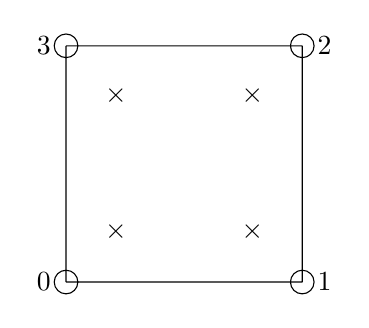
\begin{tikzpicture}[scale=1.5]

          \draw (-1,-1) circle[radius=.1] node[left=2pt]{0}-- 
          (1,-1) circle[radius=.1] node[right=2pt]{1} -- 
          (1,1) circle[radius=.1] node[right=2pt]{2} -- 
          (-1,1) circle[radius=.1] node[left=2pt]{3} -- (-1,-1);

          \draw (-.577,-.577) node{$\times$};
          \draw (.577,-.577) node{$\times$};
          \draw (.577,.577) node{$\times$};
          \draw (-.577,.577) node{$\times$};


        \end{tikzpicture}
        \caption{
          Two-point (per dimension) quadrature over the canonical
          quadrilateral element.
        }
      \end{figure}
    \end{column}
  \end{columns}
  
\end{frame}


%==============================================================
\subsection{Putting it all together}
%==============================================================
\begin{frame}{Making it look like code}
  \begin{itemize}
  \item
    The weak form of PDEs can be (with a little practice) written
    almost directly into code
  \item
    The goal is to write the integrals in a matrix-vector form
    \begin{align*}
      \int_{\Omega_0} \nabla v \cdot \nabla u \mathrm{det}\tensor{J}\dV_0 &\approx
      \int_{\Omega_0} \left(\sum_A \frac{\partial N^A}{\partial \tensor{x}} v^A\right) 
      \cdot \left(\sum_B \frac{\partial N^B}{\partial \tensor{x}} u^B\right) 
      \mathrm{det}\tensor{J}\dV_0
    \end{align*}
  \item
    Exploit linearity:
    \begin{align*}
      (v^A)^T\left(\sum_A \sum_B \int_{\Omega_0} \frac{\partial N^A}{\partial \tensor{x}} 
      \cdot \frac{\partial N^B}{\partial \tensor{x}}
      \mathrm{det}\tensor{J}\dV_0 \right) (u^B)
      &= \vec{v}^T \tensor{K}_e \,\vec{u}_e
    \end{align*}
  \end{itemize}
\end{frame}


\section{YAFEL Library}
\lstset{
  language=C++,
  basicstyle=\small\ttfamily,
  commentstyle=\color{red},
  keywordstyle=\color{blue},
  breaklines
}


%===========================================================
\subsection{General Workflow}
%===========================================================
\begin{frame}{YAFEL workflow for steady-state problem}
  \begin{itemize}
  \item
    Problem Setup
    \begin{itemize}
    \item Read/create geometry
    \item Specify boundary conditions
    \item Define problem-specific parameters (eg: material properties)
    \item Allocate persistent/problem-global data structures
    \end{itemize}
  \item
    Assemble element residuals/tangents
  \item
    Apply boundary conditions \& solve system
  \item
    Write output
  \end{itemize}
\end{frame}

\begin{frame}{YAFEL workflow for implicit time-dependent problem}
  \begin{itemize}
  \item
    Problem Setup
    \begin{itemize}
    \item Read/create geometry
    \item Specify boundary conditions
    \item Define problem-specific parameters (eg: material properties)
    \item Allocate persistent/problem-global data structures
    \end{itemize}
  \item
    Time loop
    \begin{itemize}
    \item
      Assemble element residuals/tangents
    \item
      Apply boundary conditions, solve system, update solution
    \end{itemize}
  \item
    Write output (really can do this whenever)
  \item
    Under appropriate circumstances, assembly and boundary conditions
    are moved out of the time loop, and only the linear solve/update remains
  \end{itemize}
\end{frame}

%===========================================================
\subsection{Mesh Handling}
%===========================================================
\begin{frame}[fragile]{Creating/handling Meshes}
  \begin{itemize}
  \item
    All (both) mesh types inherit from the \texttt{GenericMesh<NSD>} type
  \item
    Meshes are templated on the number of spatial dimensions
  \item
    This lets the mesh know how many components to expect for a coordinate (x, [y, [z]])
  \item
    Read mesh from Gmsh file or create a simple rectilinear mesh
  \end{itemize}

  \begin{lstlisting}[basicstyle=\small\ttfamily]
    // Read from file
    GmshMesh<3> GM(``my_mesh.msh''); 

    // Define rectilinear mesh 
    //(nodes/elements calculated, not stored)
    RectilinearMesh<3> RM(vector<double>{1,1,1}, 
                          vector<size_t>{10,10,10});
  \end{lstlisting}

\end{frame}

\begin{frame}[fragile]{GenericMesh supported operations}
  \begin{lstlisting}[]
    //Return a node
    coordinate_type node(size_t nodenum);
    
    //Return nodes comprising an element
    vector<size_t> element(size_t elnum);

    //Build list of internal faces
    void build_faces();

    //Get global node numbers of ``f''-th face of element ``e''
    vector<size_t> face_nodes(size_t e, size_t f);

    //Get iterator over mesh elements 
    MeshIterator<T> begin() const;
    MeshIterator<T> end() const;
  \end{lstlisting}
\end{frame}

\begin{frame}{Handling problem degrees of freedom}
  \begin{itemize}
  \item
    For assembly, you need a way to uniquely identify each
    degree of freedom in the global problem
  \item
    For this example problem, it's easy, because you can use
    \[
    global\_dof = node\_number
    \]
  \item
    This isn't generally the case, so the DoFManager does the mapping for you
  \item
    Currently, a basic one that works for continuous galerkin FEM
    is included in YAFEL (assuming 0-based indexing)
    \[
    global\_dof = (dof\_per\_node*node\_number) + local\_dof\_num
    \]
  \end{itemize}
\end{frame}

%===========================================================
\subsection{Elements}
%===========================================================
\begin{frame}{Element Types}
  \begin{itemize}
  \item
    All elements, regardless of geometry, have to store very similar information
  \item
    Thus, base class \texttt{Element} is used to hold this common info
  \item
    Global info
    \begin{itemize}
    \item
      Node Numbers (vector, length=nodes\_per\_el)
    \item
      Location \& weight of each quadrature point
    \end{itemize}
  \item
    At each quadrature point
    \begin{itemize}
    \item
      Value of all shape functions (Vector, length=nodes\_per\_el)
    \item
      Gradient of all shape functions wrt parent coordinates 
      (Matrix, size=(nodes\_per\_el, NSD))
    \item
      Jacobian of transformation to parent element
    \end{itemize}
  \end{itemize}
\end{frame}

\begin{frame}[fragile]{Specializing elements}
  \begin{itemize}
  \item
    To specialize an element, you must provide
    \begin{enumerate}
    \item Quadrature rule (points \& weights)
    \item Shape functions
    \end{enumerate}
  \item
    The Element class can take care of the rest
  \end{itemize}
  \begin{columns}
    \begin{column}{.6\textwidth}
      \begin{lstlisting}[basicstyle=\tiny\ttfamily]
        template<typename T>
        LinTri::shape_value(size_t node, 
                            Tensor<3,1,T> xi) {
          switch(node) {
          case 0: return 1 - xi(0) - xi(1);
          case 1: return xi(0);
          case 2: return xi(1);
          default:
            //Something is wrong!
            throw std::runtime_error(``Bad 'node' argument to LinTri::shape_value'');
          }
        }
      \end{lstlisting}
      \begin{align*}
        N^0(\tensor{\xi}) &= 1 - \xi_0 - \xi_1 \\
        N^1(\tensor{\xi}) &= \xi_0 \\
        N^2(\tensor{\xi}) &= \xi_1 \\
      \end{align*}
    \end{column}
    \begin{column}{.4\textwidth}
      \begin{figure}
        \centering
        \begin{tikzpicture}[scale=2]
          \draw (0,0) circle[radius=.05] node[below]{0}
          -- (1,0) circle[radius=.05] node[right]{1}
          -- (0,1) circle[radius=.05] node[left]{2}
          -- (0,0);

          \draw[color=gray,dashed, -latex] (0,0) -- (1.5,0) node[right]{$\xi_0$};
          \draw[color=gray,dashed, -latex] (0,0) -- (0,1.5) node[above]{$\xi_1$};
        \end{tikzpicture}
      \end{figure}
    \end{column}
  \end{columns}
\end{frame}

%===========================================================
\subsection{Assembly}
%===========================================================
\begin{frame}[fragile]{Assembly process}
  \begin{itemize}
  \item
    Assembly is at the heart of FEM, and is the process by which
    global integrals can be expressed as sums of integrals over elements
  \item
    Example code for assembling a local matrix $\tensor{K}_e$ into 
    global matrix $K_{global}$
  \end{itemize}
  \begin{lstlisting}[basicstyle=\tiny\ttfamily]

    /* Assume that an element object ``E'' exists */
    for(int A=0; A<dof_per_element; ++A) {
      int A_base = E.base(A); //element-local node number
      int A_comp = E.comp(A); //node-local dof number
      int A_g = DOFM.global_dof(elnum, A_base, A_comp);

      for(int B=0; B<dof_per_element; ++B) {
        int B_base = E.base(B); //element-local node number
        int B_comp = E.comp(B); //node-local dof number
        int B_global = DOFM.global_dof(elnum, B_base, B_comp);
        
        K_global(A_g, B_g) += K_e(A,B); // <--may not use precisely this syntax
      }
    }
  \end{lstlisting}
\end{frame}

%===========================================================
\subsection{System Solve}
%===========================================================
\begin{frame}[fragile]{Solving the system}
  \begin{itemize}
  \item
    Only need to explicitly apply the Dirichlet boundary conditions
  \item
    Neumann BCs occur naturally in formulation of weak form, so are
    handled during assembly
  \item
    In YAFEL, there is an object that handles it for you
  \item
    Object created by passing a mesh, a gmsh physical-id number, local dof component,
    and a \texttt{SpatialFunction<NSD>} 
    (an alias for \texttt{std::function<double(coordinate\_type)>})
  \end{itemize}
  \begin{lstlisting}
    DirBC bc(M, phys_id, dof_comp, 
             [](const coordinate_type &x)->double
             { return 0; });
  \end{lstlisting}
\end{frame}

%===========================================================
\subsection{Writing Output}
%===========================================================


%===========================================================
\subsection{YAFEL-isms}
%===========================================================



\section{Laplace Equation Walk-through}
\begin{frame}
  Live demo! Solving the equation we set up in example.
\end{frame}
\end{document}
%===========================================================
%===========================================================
